\section{Наблюдателни сведения за излъчващата среда}
\lfoot{}
Физиката на излъчващата в околност на свръхмасивни компактни обекти среда представлява сложна релативистка магнито-хидродинамична (GRMHD) задача, чието решаване изисква нелинейни кодове и значителен изчислителен ресурс, до каквито не-много научни групи имат достъп. Част от целите, описани в глава 1 на този труд, изискват модел на тази среда, който обаче не е нужно да произхожда \emph{директно} от GRMHD симулации. За да изследваме влиянието на пространство-времето върху реконструкцията на образа на излъчващата среда от VLBI наблюдения, е достатъчно да се формулира \emph{феноменологичен} модел тази средата, който възпроизвежда основните наблюдателни величини - пълният поток на енергия, характерният размер на образа и морфологията му. Той трябва да зададе изрази за разпределението на материята $\rho(\vec{r}\,)$, профил на скоростта ѝ $u^\mu (x^\mu)$, температурния ѝ профил $T(\vec{r\,})$ и разпределението на магнитното поле $\vec{B}(\vec{r}\,)$.\\

В общия случай строенето на подобен модел е концецптуално просто: представлява съгласуване на резултатите от наблюдения и числени GRMHD симулации, като ролята на наблюденията е да наложи ограничения върху тези симулации. Крайният резултат от това е малък брой числени модели, които са съвместими с наблюдателните данни. Тогава те могат да бъдат усредени във времето и от тях да се извлекът аналитични функции за равновесното състояния на излъчващата зона.\\ 

Бивайки концептуално проста задача, практическата ѝ реализация е силно нетривиална. Често се случва симулациите да имат значително по-голям брой свободни параметри от колкото е броят на ограниченията които могат да се наложат върху тях. Следователно и извлечените феноменологични модели (които често представляват прости степенни закони) имат свободни параметри които могат да варират значително, но пак да са съвместими с наблюденията.\\

Един от най-дълбоките и съвременни анализи oт този тип е направен от колаборацията EHT. В тази глава ще обобщим техните резултати, които се базират на наблюдения на обектите M87* и Sgr А*. Целта на изложението е да съпостави свойствата на излъчващата среда около двата обекта и да мотивира използвания от нас феноменологичен модел.
\newpage
\subsection{Основни наблюдателни резултати за M87*}

Нека концентрираме вниманието си върху два основни източника на информация, предоставени от EHT: морфологията на получените от тях образи и поляризаццията им. \\

На фигура \ref*{M87_I_Image} са показани усредените от всички методи за реконструкция образи за 4те дни на наблюдение на М87*. Както можем да видим, те имат два характерни белега:\\

$\bullet$ Силно изразена централна депресия. Тя се интерпретира като \emph{сянката} на сръхкомпактния обект. Това за пръв път позволява да се направи \emph{директна} наблюдателна оценка за масата на сръхкомпактен обект. Стойността, получена от екипа на EHT (използвайки предишни оценки за разстоянието до обекта), е $M_{М87^*} = (6.5\pm 0.7)\times 10^{9} M_\odot$.\\

$\bullet$ Асиметричен пръстен. Той е образът на излъчващата среда, изкривен през ефекта на гравитационната леща. Предполаганата причина за асиметрията е силен релативистки ефект на Доплер от едромащабното движение (т.н. \emph{bulk movement}) на плазмата.\\

\begin{minipage}{15em}
	\centering
	\includegraphics[scale = 0.5]{М87_Avg_Images.jpg}
	\captionof{figure}[Реконструиран от екипът EHT образ на М87]{Реконструирани от екипът EHT образи на М87 CITE HERE. Яркостната температура съответства на интегриран поток $\mathcal{F}_{\text{total}}\approx0.5\,\text{Jy}$}
	\label{M87_I_Image}
\end{minipage}
\begin{minipage}{16em}
	Имайки предвид измерената яркостна температура и честотата на наблюдение, предполагаемият механизъм за излъчване е релативисткото синхотронно излъчване. С това може да се даде оценка за средната плътност, големина на магнитното поле и темпа на акреция в излъчващата среда. Екипът на EHT дава следните стойности на базата на сферичен, еднозонов и изотермен модел (CITE HERE):
	\begin{equation}
		\begin{aligned}
			&n_{\text{avg}} \approx 2.9\times 10^{4} \text{cm}^{-1}\\
			&B_{\text{avg}} \approx 4.9 \text{G}\\
			&\dot{M} \approx 2.7\times 10^{-3} \text{M}_\odot \text{yr}^{-1} \approx 2 \times 10^{-5} \dot{M}_{\text{Edd}},
		\end{aligned}
	\end{equation}
	при предположена температура $T = 6.25\times 10^{10}$ K и $\dot{M}_{\text{Edd}}$ е темпът на акреция, който би произвел светимост, равна на светимостта на Едингтън. 
\end{minipage}\\

Тук трябва да се направи важен коментар за тези стойности. Те са в съгласие с предсказанията на \emph{оптически тънки} GRHMD модели в режим на \emph{радиационна неефективност} (и с предишни оценки на динамичното състояние на средата CITE HERE). Характерното за тези модели е, че Кулоновата обмяна на кинетична енергия между електрони и йони в плазмата е силно потиснато от ниската плътност и високата температура (понеже радиуса на Дебай скалира като $r_D \propto T^{-1/2}$). Тъй като електроните излъчват синхотронно своята енергия много по-бързо от йоните$^1$, потиснатата обмяна на енергия означава, че ансамблите от електрони и йони се намират при значително различни температури. Тогава трябва да допуснем, че оценката за плътност и температура от (3.1) се отнася само за ансамбъла от електрони.\\

Друго важно нещо, което трябва да се отбележи, е че възпроизвеждането на морфологията и потока на фигура \ref{M87_I_Image} може да се осъществи чрез варирането на кой да е от параметрите $\{n_{e},\,T_{e},\, \vec{B}\}$ - т.е. само с ограничения от морфологията на пълният интензитет, тези стойности в моделите се израждат. Затова по-точна оценка за параметрите на излъчващата среда се изискват допълнителни ограничения от наблюденията. Такива могат да дойдат от \emph{поляризацията} на лъчението. На фигура \ref{M87_Pol_Image} са показани резултатите на EHT от \emph{поляризираните} наблюдения на M87*, публикувани 2 години по-късно.\\

 \begin{figure}[h!]{
 \centering
 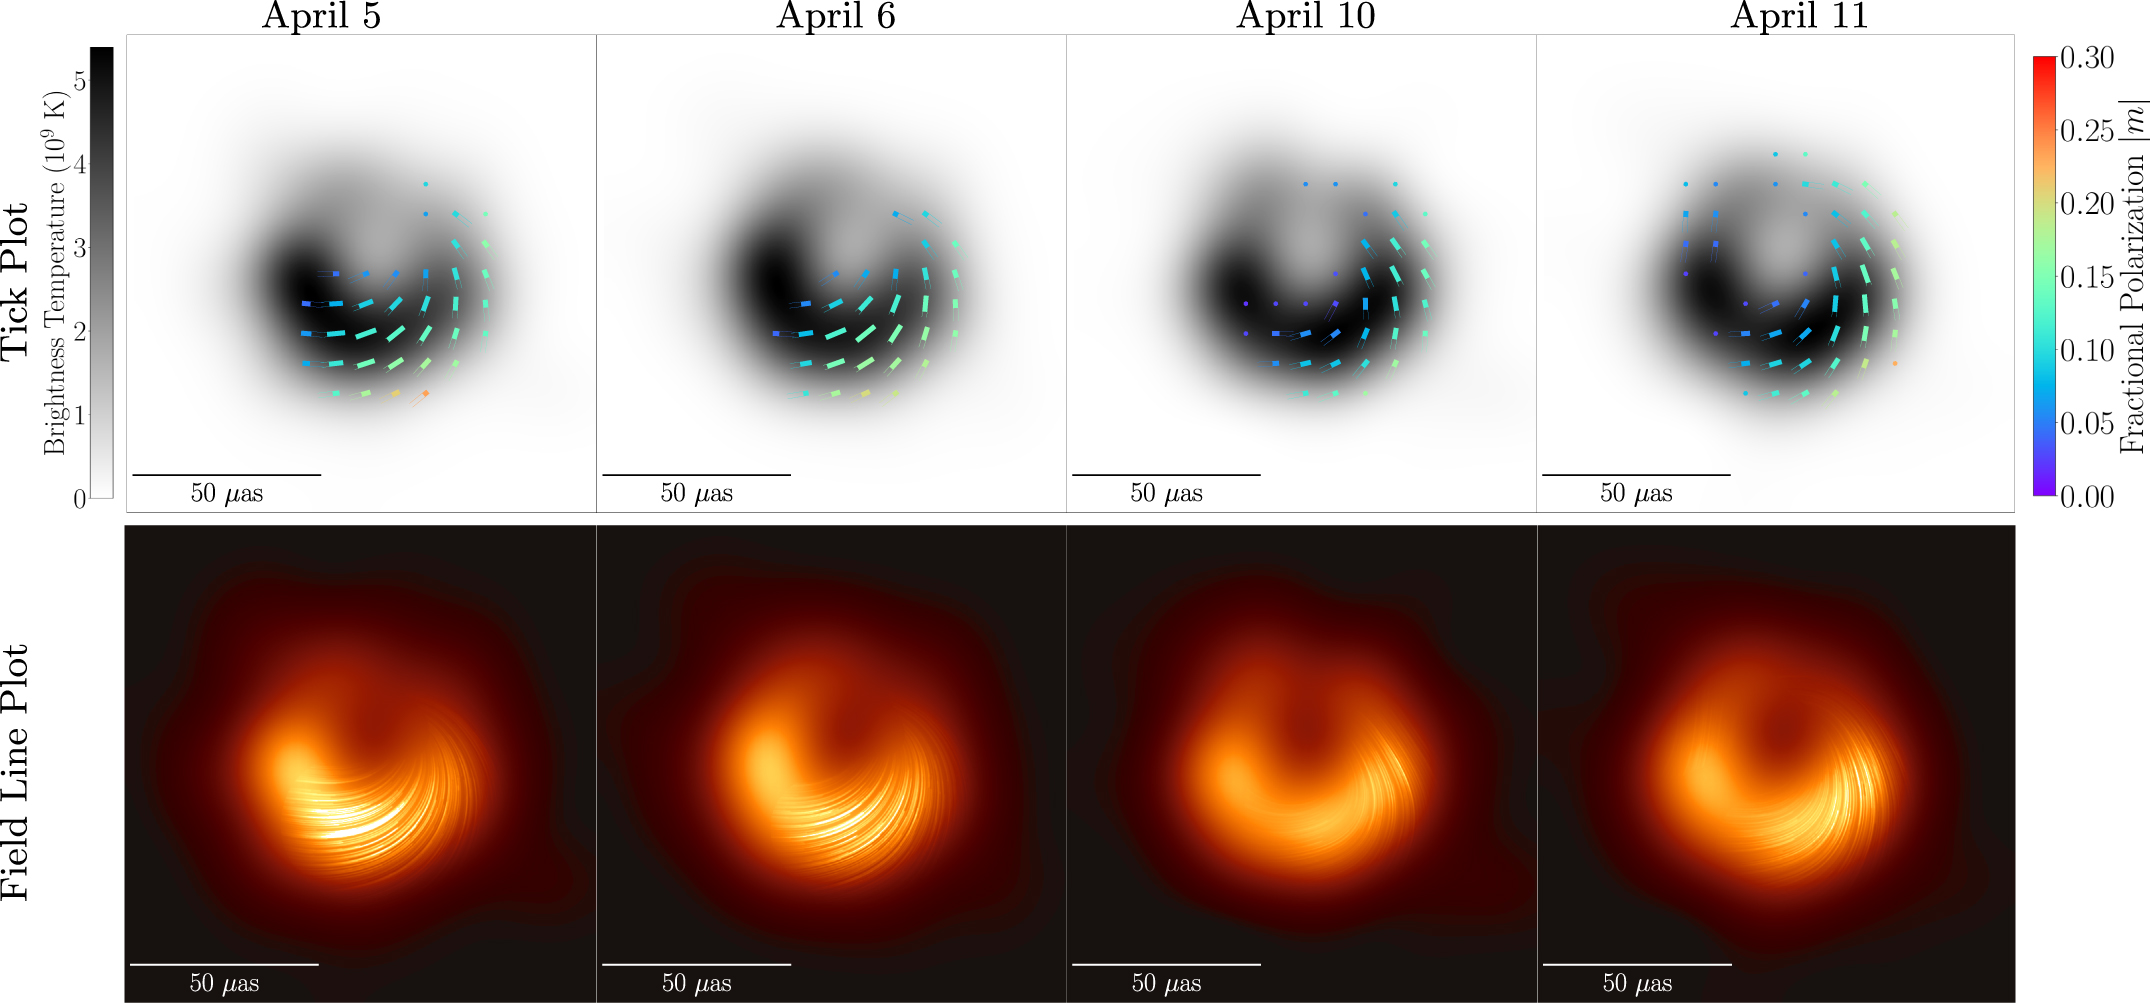
\includegraphics[scale = 0.7]{M87_Polarization_overlay.jpg}\newline
 \captionof{figure}[Реконструиран от екипът EHT поляризиран образ на М87]{Реконструирани от екипът EHT поляризирани образи на М87 CITE HERE. Средната относителна линейна поляризация варира през времето на наблюдение в интервала $5.7\% \le \braket{|m|} \le 10.7\%$. Долните фигури третират поляризацията като векторно поле, и я визуализират върху образите от фигура \ref{M87_I_Image}.} 
 \label{M87_Pol_Image}}
 \end{figure}
 \setlength{\footskip}{20pt}
 \lfoot{
 	\noindent\makebox[\linewidth]{\rule{\textwidth}{0.4pt}}
 	$^1$ Излъчената от заредени частици електромагнитна енергия е пропорционална на квадрата на ускорението. При разглежданите температури можем да приемем, че средата е напълно йонизирана. Предполагайки химичен състав предимно от водород, можем да приемем, че $|q_{\text{ion}}| = e$ и следователно отношението на мощността на излъчване от двата ансамбъла ще бъде $\frac{P_{\text{ion}}}{P_e} \approx \left(\frac{m_e}{m_{\text{ion}}}\right)^2 \ll 1$
 }
 
 Виждаме от фигура \ref{M87_Pol_Image}, че относителната линейна поляризация на образа е много-по малка от характерната за синхотронното излъчване $\lbrace |m| \rbrace_\text{synch}\approx 0.7$. Основните физични механизми, които могат да предизвикат това в оптически тънка среда са два:\\\newline
 $\bullet$ Фарадеево въртене на вектора на поляризацията \emph{вътре} в самата излъчваща среда. Приемаме, че това се случва в средата, понеже наблюдаваме самата галактика при $\approx 20\,\text{deg}$ инклинация спрямо нейната равнина, и лъчът на зрението към нея не минава през значителна част от Млечният път - следователно няма значително количество материя по лъча на зрение \emph{извън} излъчващата среда.\\
 $\bullet$ Турбуленция в структурата на магнитно поле.\\\newline
И двата ефекта биха предизвикали силна вариация във вектора на поляризацията на малки разстояния по образа, която след усредняване по ефективната резолюция на телескопа, приблизително се нулира. Екипът на EHT е извършил анализ върху относителният принос на тези два механизма в CITE HERE. Те показват, че турбуленцията сама по себе си не е достатъчна за да възпроизведе ниската средна поляризация на образите. Доминантният принос има Фарадеевото въртене. Тогава може да се направи оценка за \emph{Фарадеевата оптическа дълбочина} CITE HERE VII
\begin{equation}
	\tau_{\rho_V} = \int \rho_{V}(r)dr\approx 5.2\left(\frac{r}{5r_g}\right)
\end{equation}
\lfoot{}

Екипът на EHT тогава използва условието $\tau_{\rho_V}>2\pi$ за допълнително ограничение върху еднозоновия, сферичен и изотермен модел от CITE HERE V за да даде следните допустими стойности на параметрите на физичната среда:

\begin{equation}
	\begin{split}
		10^{10} \le\,\, &T_e \le 1.2 \times 10^{11}\,\text{K}\\
		1 \le\,\, &B \le 30\, \text{G}\\
		10^4 \le\,\, &n_e \le 10^7 \text{cm}^{-3}
	\end{split}
\end{equation}

В техните разглеждания, стойности $B \gg 30$ G водят до значителна кръгова поляризация, каквато не се наблюдава във фигура \ref{M87_Pol_Image}, докато стойности $B > 5$ G са достатъчни за генериране на джетове с мощност $P_{jet} > 10^{42}\,\text{erg s}^{-1}$, каквато се наблюдава за M87*.\\

Като последна стъпка от анализа си, екипът на EHT разгледа голям брой изображения, генерирани на базата на GRMHD симулации и разработва набор от тестове, с помощта на които съди съвместимостта на дадена симулация с наблюденията им. Свободните параметри на изображенията са:\\\newline
$\bullet$ Параметрите на GRMHD симулациите - параметърът на въртене $a_*$ и безразмерният магнитен поток през хоризонта на събитията $\phi = \frac{\Phi_{BH}}{\dot{M}r_g^2c}$. Вторият количествено разделя режима на акреция между двата най-често разглеждани модела - Стандартна и Нормална Еволюция (SANE) и Магнитно Задържан Диск (MAD). Симулациите са направени при колинеарни и анти-колинеарни вектори на момента на импулса на плазмата и черната дупка. Адиабатните кофициенти на плазмата $\gamma$ са фиксирани на 4/3 за SANE и 13/9 за MAD.\\\newline
$\bullet$ Отношението на йонната към електронната температура $R$. Понеже GRMHD еволюира плътността на пълната вътрешната енергия, а не на отделните ансамбли, $T_e$ се задава на базата на параметрите $\beta = p_{\text{gas}} / p_\text{mag}$, $R_\text{high}$, и $R_\text{low}$. Тогава $T_e$ се пресмята като CITE EHT VIII:
\begin{equation}
	R = R_\text{high}\frac{\beta^2}{1 + \beta^2} + R_\text{low}\frac{1}{1 + \beta^2},\quad T_e = \frac{2m_pu_\text{gas}}{3\rho k (2 + R)},
\end{equation}   
където разпределението на електроните по енергии е прието за изцяло топлинно. В CITE EHT VIII HERE са разгледани следствията от добавяне на електронен ансамбъл, разпределен по степенен закон.\\\newline
$\bullet$ Инклинацията на наблюдателя.\\

Процедурата по сравняване на тези симулации с наблюденията е описана в CITE EHT V AND VIII. Накратко тя представлява налагане на условия (т.е. тестове), базирани както на наблюденията на EHT, така и на исторически такива в радио и рентгеновата област, наблюдения на джета, както и условия изхождащи от общи физични принципи (например, че излъчващата среда трябва да е достигнала равновесно състояние). Заключението от този анализ е, че най-вероятният режим на акреция, който възпроизвежда наблюденията (т.е. преминава успешно тестовете), е MAD при $a_*\ne 0$, с предимно полоидално магнитно поле и $R_\text{high} > 10$. 


\subsection{Основни наблюдателни резултати за Sgr A*}

Наблюденията на Sgr A*, и оценяването на структурата на излъчващата са значително по-тежки задачи от колкото за M87* (въпреки по-малкото разстояние!). Релевантните за нас причини са:\\\newline
$\bullet$ Наблюденията се извършват през цялата дълбочина на галактичният диск. Това внася значителни неопределености в оценката на физичните свойства на излъчващата среда. Най-релевантната от които е Фарадеевото въртене от материя, \emph{извън} излъчващата среда, по лъча на зрението.\\\newline
$\bullet$ Sgr A* показва значително по-голяма променливост. Ако приемем периода на ISCO орбитите, като характерна динамична скала, тогава (предполагайки черна дупка на Кер) имаме $t_{d,M87^*} \approx 5 $ дена за prograde орбитите, докато $t_{d,Sgr A^*}\approx 4 \text{min}$. Имайки предвид, че почти всичкото излъчване, наблюдавано от EHT, идва от материя в околност на тези орбити, структурата на излъчващата среда може да се промени драстично, дори по време на наблюденията. \\\newline
$\bullet$ Липсата на силно изразен джет, който да се използва за оценка на наблюдателната инклинация и допълнително ограничение върху режима на акрецията.\\\newline
Променливостта можем директно да видим отразена в реконструкциите на EHT:\\

\begin{minipage}{15em}
	\centering
	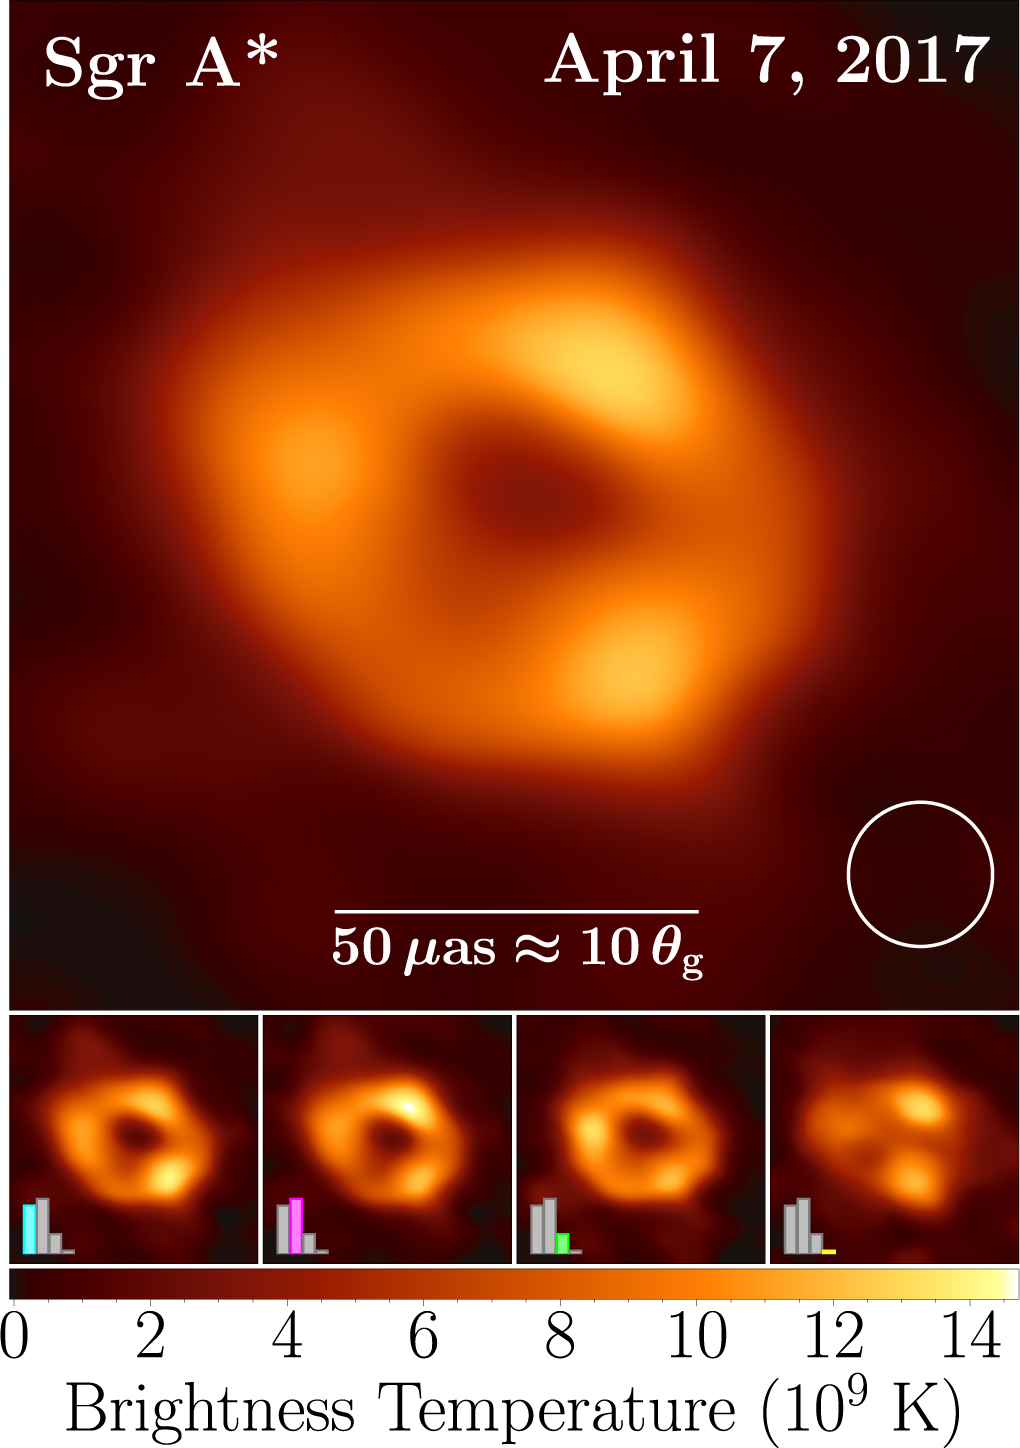
\includegraphics[scale = 0.5]{SgrA_Avg_Images.jpg}
	\captionof{figure}[Реконструиран от екипът EHT образ на Sgr A$^*$]{Реконструирани от екипът EHT образи на Sgr A$^*$ CITE HERE. Яркостната температура съответства на интегриран поток $\mathcal{F}_{\text{total}}\approx2.4\,\text{Jy}$}
	\label{SgrA_I_Image}
\end{minipage}
\begin{minipage}{16em}
Виждаме, че образите притежават основните белези на тези от M87$^*$ (т.е. пръстеновидна структура и централна депресия на интензитета), но също и множество "горещи" петна. Те са директен белег на променливостта на излъчващата среда, но (както коментира екипа в CITE EHT HERE) азимуталната структура на тези петна не е добре ограничена от наблюденията. Върху тези образи може да се приложи същият анализ за груба оценка на основните параметри на средата и самия централен обект CITE EHT HERE:
\begin{equation}
	\begin{aligned}
	M_{\text{Sgr A}^*} &= 4\times 10^6 M_\odot\\
	n_{\text{avg}} &= 10^6\, \text{cm}^{-3}\\
	B_{\text{avg}} &= 29\, \text{G}
	\end{aligned}
\end{equation}
\end{minipage}\\

Тези стойности (заедно с яркостната температура), както при M87$^*$, поставят излъчващата среда в оптически тънък и радиационно неефективен режим. Следователно екипът на EHT отново извършва съпоставка с набор от GRMHD симулации CITE EHT HERE. Те използват \emph{комбинирани} наблюдения в радио, близката инфрачервена и рентгенова област, извършени в рамките на няколко дни от основните EHT наблюдения за да изработят 11 морфологични ограничения върху симулациите, които за разлика от тези за M87$^*$ включват и ограничения върху променливостта. Резултатът от анализът заслужава особено внимание:\\

Нито един модел на удовлетворява всички ограничения, следващи от комбинираните наблюдения! Най-ограничаваща се оказва променливостта - набора GRMHD симулации не възпроизвеждат по задоволителен начин променливостта на Sgr A$^*$. В CITE EHT HERE са обсъдени потенциални причини за това - от гледна точка на неразделена променливост в наблюденията, и от страна на отчитането на безколизната термодинамика на електроните в симулациите.\\\newline
Ако бъде отслабено изискването за възпроизвеждане на променливостта, моделите които най-добре описват комбинираните наблюдения са отново (както при М87$^*$) MAD при $a_*>0$, ниска инклинация $i = 30^\circ$ и с високо $R_\text{high} = 160$. Фактът, че два независими обекта в ядрата на две различни по размер галактики, притежават излъчваща среда която се намира в сходен физически режим подсказва за \emph{универсалност} на процесите покрай свръхмасивни компактни обекти. Този резултат е потвърден от наскоро публикуваният анализ на поляризираният образ на Sgr A$^*$ CITE EHT HERE, представен на фигура \ref{SgrA_Pol_Image}.\\

\begin{minipage}{18em}
	Използвайки отново еднозонов, изотермен модел със стойностите (3.5), може да се даде оценка за Фарадеевата оптическа дълбочина CITE EHT HERE:
	\begin{equation}
		\tau_{\rho_V} = \int \rho_{V}(r)dr\approx 0.98\left(\frac{r}{5r_g}\right).
	\end{equation}
	Сравнявайки стойностите за $\tau_{\rho_V}$ и $\braket{|m|}$ между M87$^*$ и Sgr A$^*$ виждаме, че е изпълнено следното условие:
	\begin{equation}
		\frac{\tau_{\rho_V}^{\text{M87}^*}}{\tau_{\rho_V}^{\text{Sgr A}^*}}\approx\frac{\braket{|m|}^{\text{Sgr A}^*}}{\braket{|m|}^{\text{M87}^*}},
	\end{equation}
	което подкрепя интерпретацията, че Фарадеевото въртене играе важна роля във формирането на тези образи. Имайки предвид, че наблюдаваме Sgr A$^*$ през равнината на галактическият диск, е възможно значителна част от това въртене да е причинено \emph{извън} излъчващата среда (от т.н. външен Фарадеев екран).
\end{minipage}$\,\,\,$
\begin{minipage}{15em}
	\centering
	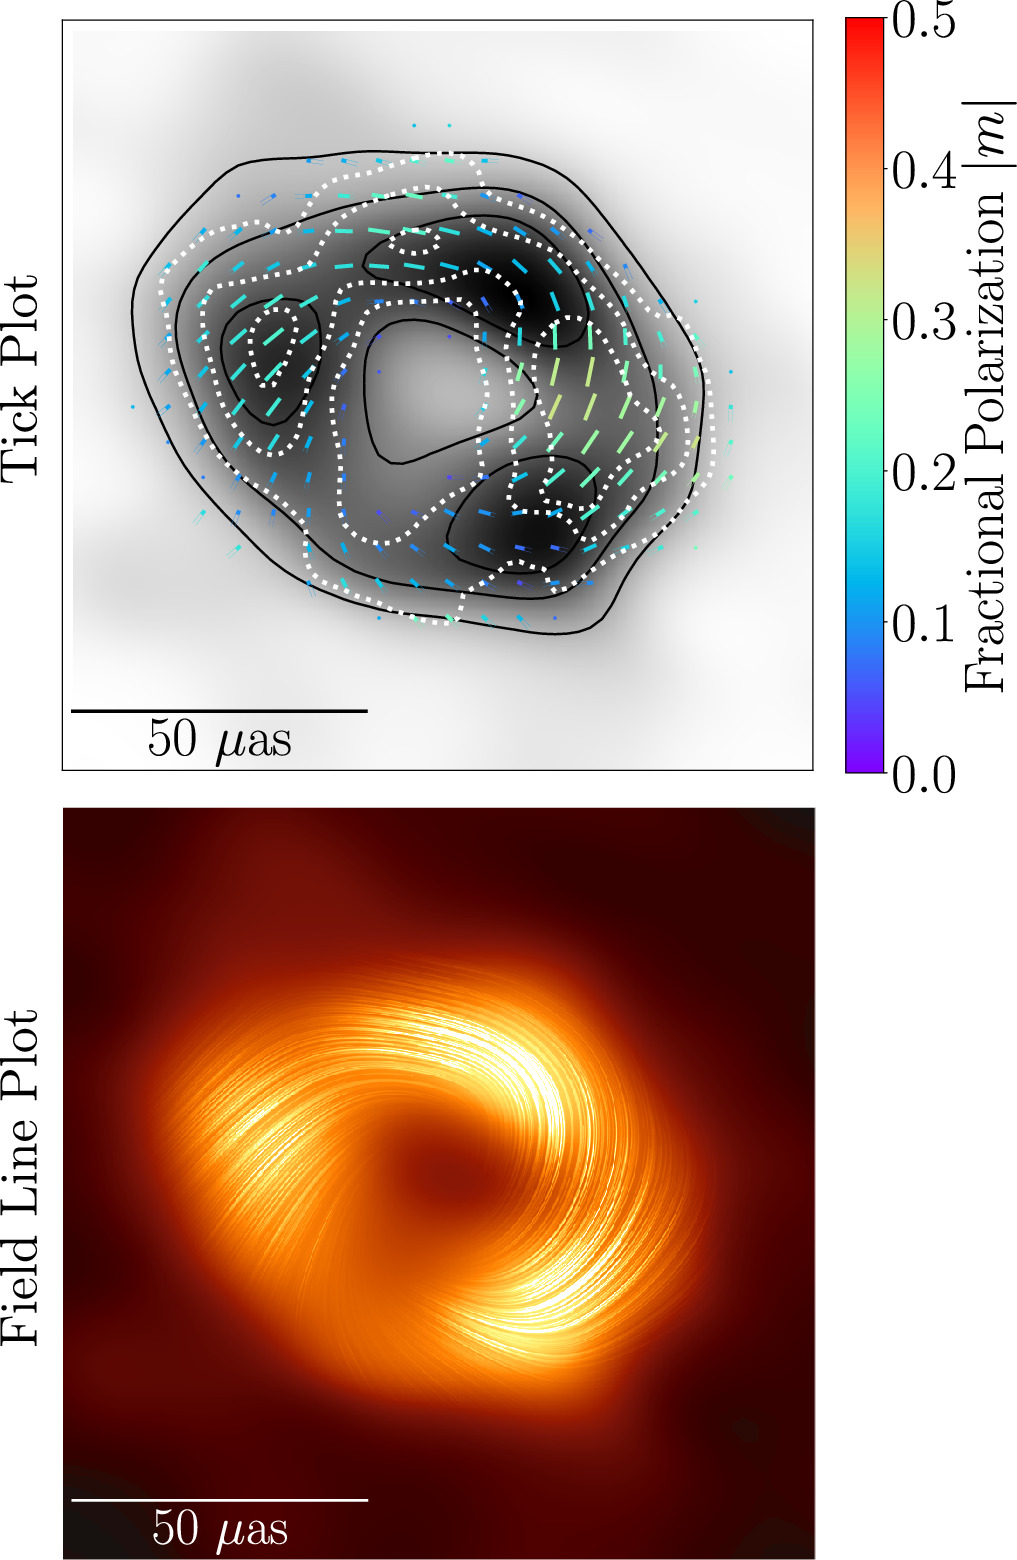
\includegraphics[scale = 0.5]{Sgr_A_Polarization_overlay.jpg}
	\captionof{figure}[Реконструиран от екипът EHT поляризиран образ на Sgr A$^*$]{Реконструиран от екипът EHT поляризиран образ на Sgr A$^*$ CITE HERE. Средната относителна линейна поляризация e оценена в интервала $24\% \le \braket{|m|} \le 28\%$ CITE EHT VIII HERE.}
	\label{SgrA_Pol_Image}
\end{minipage}\\

Хипотезата за съществуване на външен екран е подкрепена от съпоставка с GRMHD модели - ако предположим, че всичкото Фарадеево въртене е причинено от самата излъчваща среда, екипът на EHT не намира \emph{нито един} GRMHD модел, който може да възпроизведе фигура \ref{SgrA_Pol_Image}. Несъответствието се изразява в това, че моделите не възпроизвеждат т.н. \emph{мярка на въртенето} (RM$^1$), дефинирана като:
\begin{equation}
	\text{RM} = \frac{d\chi}{d\lambda^2},
\end{equation}
където $\chi$ e позиционният ъгъл на вектора на електричното поле, върху образа и $\lambda$ e дължината на вълната. Симулациите естествено възпроизвеждат \emph{големината} на RM, но не и променливостта ѝ. Дългогодишни наблюдения на Sgr A$^*$ показват, че RM търпи силна променливост по големина, но знакът ѝ никога не се променя. От друга страна всички модели, разгледани от екипа на EHT, показват смяна на знака на RM всеки няколко \emph{часа} CITE EHT HERE. Това несъответствие може да се обясни ако се приеме, че:\\\newline
$\bullet$ Силната променливост на RM се дължи на характерната променливост на излъчващата среда в околност на свръхкомпактния обект.\\\newline
$\bullet$ Константният знак на измерените стойности на RM се дължи на външен и \emph{непроменлив} Фарадеев екран.\\

Ако се приеме тази хипотеза, може да се отчете ефекта на външният екран, и образите от фигура \ref{SgrA_Pol_Image} могат да бъдат коригирани са сравнение с GRMHD моделите CITE EHT HERE AND OTHER. Резултатът от това сравнение е, че екипът на EHT изолира един единствен GRMHD модел, който е съвместим с образите от фигура \ref{SgrA_Pol_Image} - MAD с $a_* = 0.94$, $R_\text{high} = 160$ и наблюдателна инклинация $i = 150^\circ$ със съосни вектори на момента на импулса на плазмата и черната дупка.
 \setlength{\footskip}{0pt}
\lfoot{\noindent\makebox[\linewidth]{\rule{\textwidth}{0.4pt}}\\
$^1$ Дефиницията на RM e мотивирана от това, че уравнение (2.27), при липса на поглъщане и излъчване $\kappa = \mathcal{J} = 0$, както и пренебрежимо мискиране между линейна и кръгова поляризация $\rho_Q = 0$ предсказва, че линейно поляризирана вълна би претърпяла завъртане на нейният електричен вектор на ъгъл $\Delta\phi = \frac{e^3\lambda^2}{2\pi m_e^2 c^4}\int n(s)B_\parallel(s) ds$ CITE HERE, където $s$ e дължина, измерена по траекторията на лъча и $B_\parallel$ e колинеарната с вълновия вектор компонента на магнитното поле. Дефинирайки RM като (3.8), ние изолираме екефта на средата.}